\chapter{Voice Assistance}

We spend so much time using devices that have integrated voice assistants that we usually forget how incredibly fast they have
evolved. Nowadays, they can recognize thousands of words and expressions really fast, and they are even capable to imitate
emotions. What is more, they fit in a pocket. But the reality was totally different just a couple of decades ago. From the IBM
Shoebox to Siri, in this chapter I will explore the fundamentals of voice assistance.

\section{What is voice assistance?}
Voice assistance is the result of another form of interaction between humans and computers.\cite{botsocietyVUI} The Voice User
Interface (VUI), which has the voice assistants as a result, allows a user to interact with computer or mobile or other electronic 
devices through speech or voice commands. Thus, VUI is an interface of any speech recognition applications.

Therefore, a voice assistance, also known as virtual assistant, is an application program that understands natural language voice 
commands and can perform tasks or services for an individual. Its expansion has been truly remarkable in the last few years, to the
point that we can see devices that exclusively work as virtual assistants, with integration with many other services. Its real usefulness
in society, though, remains to be seen, as this field is commonly viewed with skepticism and mistrust, and the fact of talking to a 
machine as if it were another human being remains an obstacle to overcome.

As I mentioned, voice assistants are now present in plenty of platforms:

\begin{itemize}
	\item \textbf{Smart speakers:} Google Home, Apple HomePod, Amazon Echo, Movistar Home.
	\item \textbf{Mobile operating systems:} such as Siri in iOS, Google Assistant in Android, Bixby on Samsung phones.
	\item \textbf{Desktop operating systems:} Siri on macOS and Cortana on Windows 10.
	\item \textbf{Smartwatches} 
	\item \textbf{TVs:} Siri on Apple TV and the assistants in Samsung Smart TVs.
	\item \textbf{Inside mobile apps:} EVO Assistant in the mobile application of the Spanish bank EVO.
\end{itemize}

\begin{figure}
	\centering
	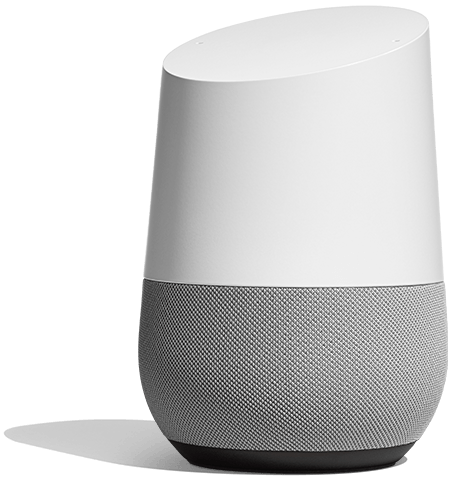
\includegraphics[width=0.5\textwidth]{images/Chapter_03/google-home.png}
	\caption{Google Home, a smart speaker integrated with the Google Assistant}
	\label{fig:google-home}
\end{figure}

\begin{figure}
	\centering
	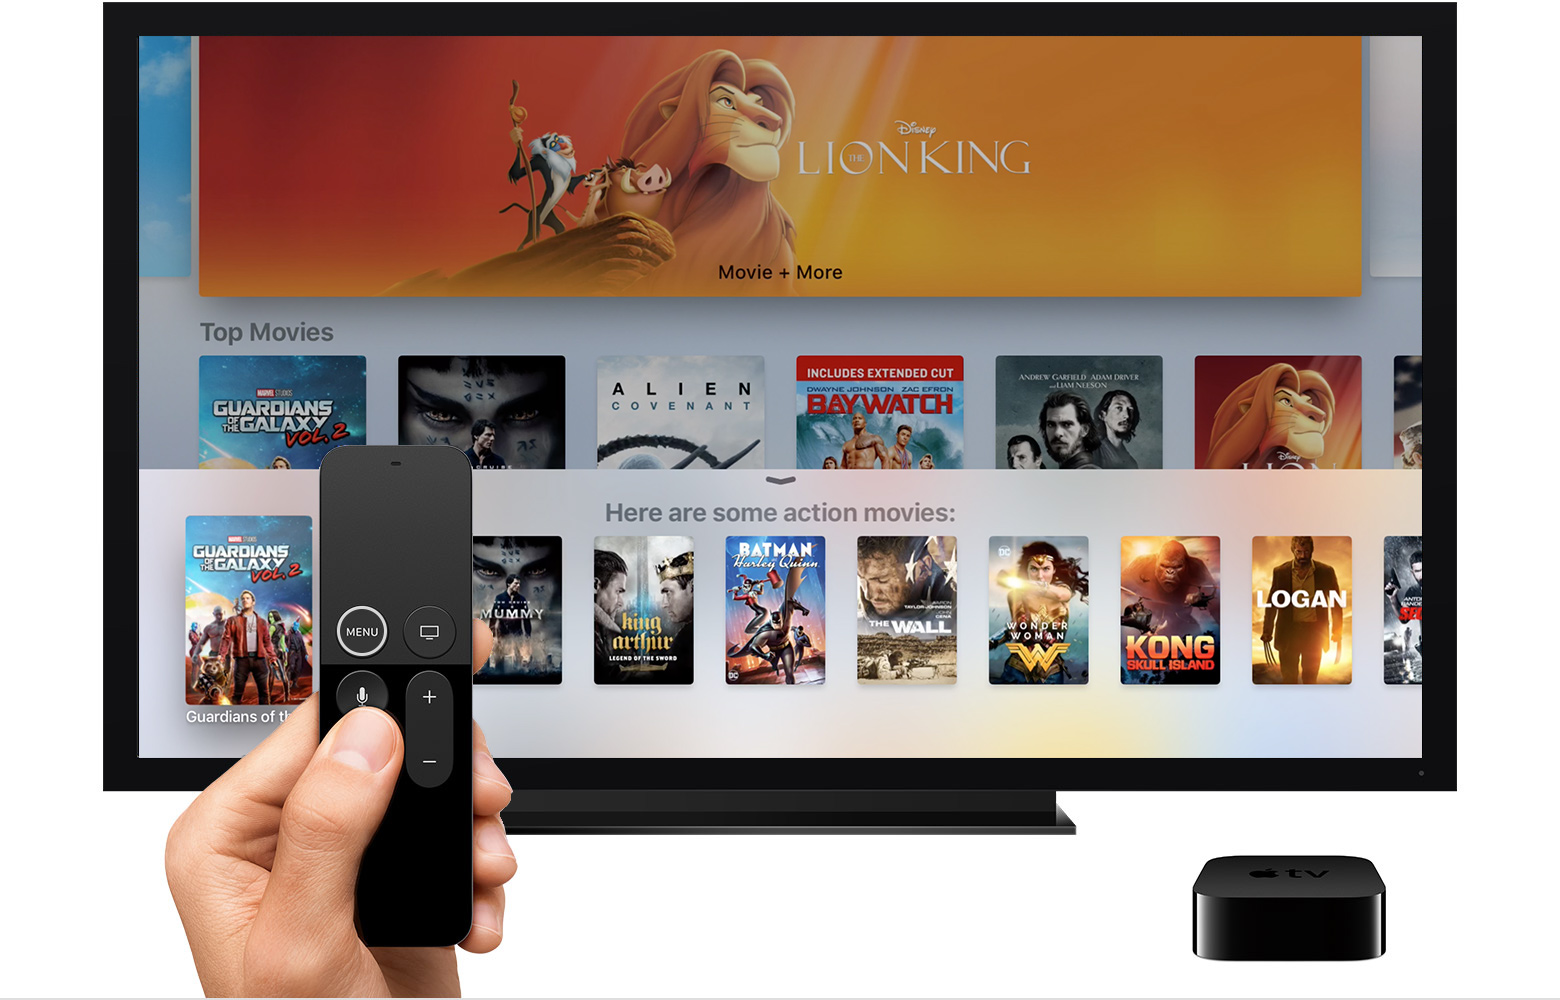
\includegraphics[width=0.9\textwidth]{images/Chapter_03/apple-tv.jpg}
	\caption{Apple TV and the Siri Remote, which has a microphone to interact with Siri}
	\label{fig:apple-tv}
\end{figure}

The history of voice assistance goes back to 1961, when IBM introduced the IBM Shoebox.\cite{voicebotTimeline} 
This was a very innovative product at that moment. Although it was not suitable for commercial use, it did mark the 
beginning of a revolution, the fruits of which we can now see. 

The Shoebox was capable of recognizing 16 spoken words, including ten digits from 0 through 9. When a number and 
command words such as \textit{plus}, \textit{minus} and \textit{total} were spoken, Shoebox instructed an adding machine 
to calculate and print answers to simple arithmetic problems. It classified the electrical impulses generated from a microphone
according to various types of sounds and activated the attached adding machine through a relay system.\cite{ibmArchivesShoebox}

Later on, there were more attempts from the research field, as the HARPY Speech Recognition System from the Carnegie
Mellon University, in 1976.\cite{lowerre76} Is could recognize about 1000 words.

Nevertheless, it was not until 1990 that the first speech recognition for consumers appeared: the Dragon Dictate. Seven years
later, the same company presented the Dragon NaturallySpeaking, which introduced continuous speech recognition as a novelty.






